\chapter{De las partículas a un campo cuántico sencillo}

Construyamos de nuevo el campo cuántico sencillo, pero desde un ángulo algo distinto. Hay dos caminos para llegar a la teoría cuántica de campos. Podemos partir de las partículas y descubrir por qué un campo es el lenguaje natural para describirlas, o partir de un campo ondulatorio y descubrir por qué sus excitaciones aparecen en cuantos. Ambos caminos son útiles. Aquí seguiremos el primero.

La mecánica cuántica ordinaria puede describir una partícula, dos partículas o cualquier otro número fijo. La naturaleza no respeta esa restricción. El número de fotones en una habitación cambia cada vez que las luces emiten o absorben radiación. Las partículas inestables se desintegran. Por ejemplo, en la desintegración beta,
\begin{equation}
n\longrightarrow p+e^-+\bar{\nu}_e,
\end{equation}
cambian a la vez las poblaciones de varias especies de partículas. Por eso queremos una mecánica cuántica lo bastante amplia para incluir todos los números de ocupación posibles y, con el tiempo, los procesos que permiten pasar de unos a otros.

Por ahora simplificaremos drásticamente. Hay una sola especie de partículas no relativistas. Primero ampliaremos su espacio de estados para que pueda contener cualquier número de partículas y solo después hablaremos de más especies, relatividad, dispersión y desintegración. Ninguna de las matemáticas es especialmente difícil, pero el cambio de perspectiva es abstracto. Conviene avanzar despacio para que la notación no oculte la idea.

\section{El punto de partida: una partícula}

Empecemos con una sola partícula en el estado \(|\psi\rangle\). Su función de onda en el espacio de posiciones es
\begin{equation}
\psi(x)=\langle x|\psi\rangle.
\label{eq:l07-wavefunction}
\end{equation}
Esta \(\psi\) minúscula es una función ordinaria con valores complejos. Todavía no es un campo cuántico ni un operador que actúe sobre un espacio de estados de muchas partículas.

La regla de Born dice que
\begin{equation}
\rho_\psi(x)=|\psi(x)|^2=\psi^*(x)\psi(x)
\label{eq:l07-born-density}
\end{equation}
es la densidad de probabilidad de encontrar la partícula en \(x\). Para un estado normalizado,
\begin{equation}
\int dx\,\psi^*(x)\psi(x)=1.
\label{eq:l07-one-particle-normalization}
\end{equation}
El miembro derecho es la probabilidad total. Como este problema contiene exactamente una partícula, también resulta ser el número de partículas. Esa coincidencia será una pista útil, aunque aquí sea trivial.

\begin{classroomqa}
\lecturetimestamp{00:09:13}
\audiencequestion{¿Por qué debe tener la densidad de probabilidad la forma \(\psi^*(x)\psi(x)\)?}
\lecturerresponse{Esa es la regla de Born, uno de los postulados de la mecánica cuántica. La amplitud correspondiente al resultado de posición \(x\) es \(\langle x|\psi\rangle\); la densidad de probabilidad es su módulo al cuadrado. No se deriva de la construcción de campos que veremos más adelante.}
\end{classroomqa}

\section{Modos, ortogonalidad y completitud}

Hay muchas bases útiles para el espacio de Hilbert de una partícula. Los estados propios de posición forman una base. Los estados propios de cualquier operador hermítico forman otra, con las salvedades habituales para los espectros degenerados y continuos. Como pronto nos interesará la energía, elijamos un conjunto completo y ortonormal de estados propios de energía de una partícula:
\begin{equation}
|1\rangle,\ |2\rangle,\ldots,
\qquad
\psi_i(x)=\langle x|i\rangle.
\end{equation}

Una partícula en una caja permite concretar el índice \(i\). La función de onda del estado fundamental no tiene nodos interiores; la del siguiente estado tiene uno, y las de los estados superiores oscilan con más rapidez. En esencia, son ondas sinusoidales de un pozo cuadrado infinito ideal.

\begin{figure}[htbp]
\centering
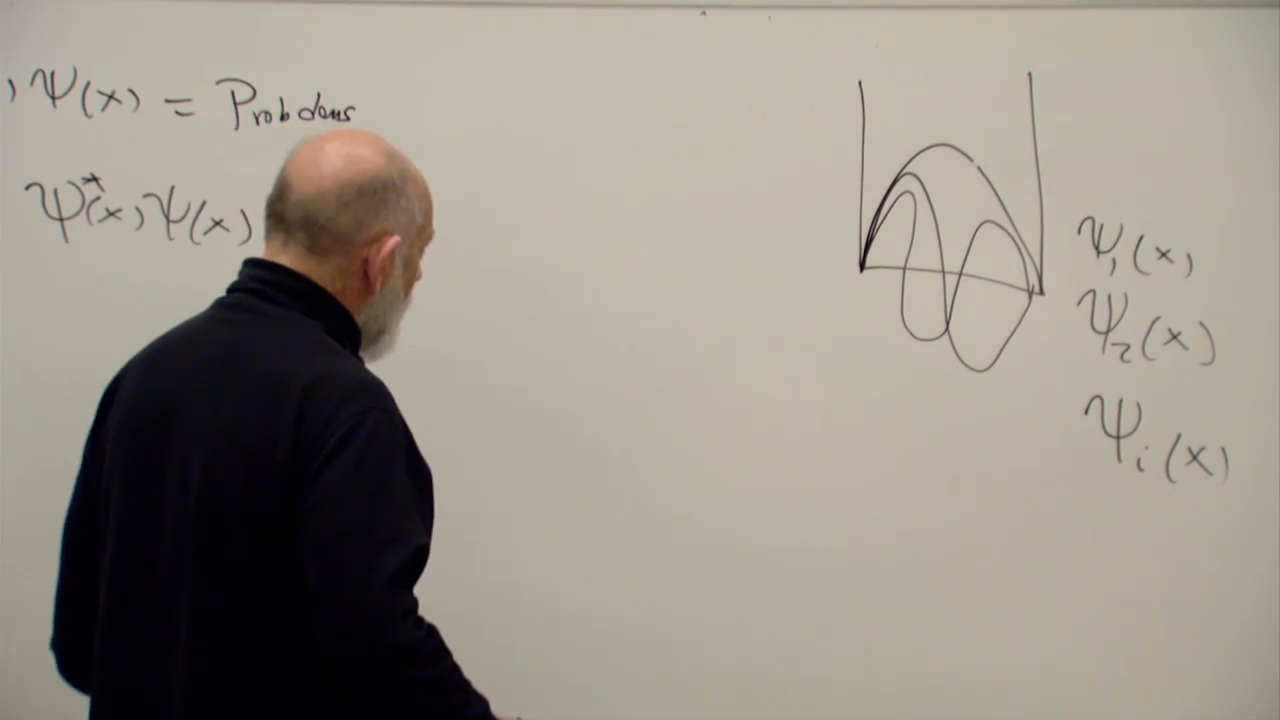
\includegraphics[width=0.94\linewidth]{lecture_07_frame_01.png}
\caption{Los modos de la caja en la pizarra de la clase. A la izquierda se ven restos de la densidad de Born de una partícula y de su normalización; a la derecha, el pozo muestra \(\psi_1(x)\), \(\psi_2(x)\) y la etiqueta general \(\psi_i(x)\).}
\lectureframe{00:08:25}
\end{figure}

La misma estructura de modos puede separarse de lo que oculta la pizarra en directo:
\begin{figure}[htbp]
\centering
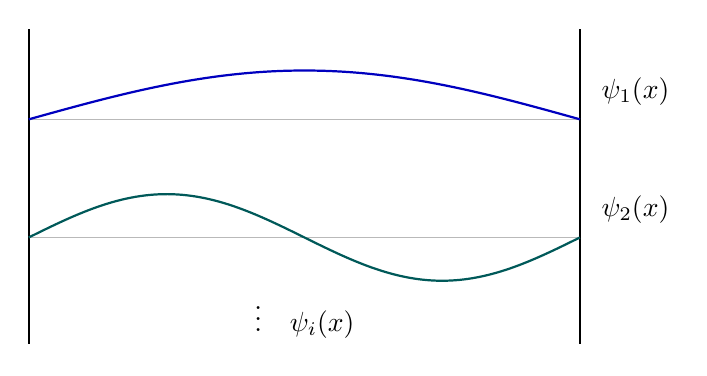
\begin{tikzpicture}[x=1cm,y=1cm]
  \draw[thick] (0,0) -- (0,4.0);
  \draw[thick] (7,0) -- (7,4.0);
  \draw[gray!55] (0,2.85) -- (7,2.85);
  \draw[gray!55] (0,1.35) -- (7,1.35);
  \draw[blue!75!black,thick,domain=0:7,samples=120]
    plot (\x,{2.85+0.62*sin(180*\x/7)});
  \draw[teal!70!black,thick,domain=0:7,samples=120]
    plot (\x,{1.35+0.55*sin(360*\x/7)});
  \node[right] at (7.15,3.20) {$\psi_1(x)$};
  \node[right] at (7.15,1.70) {$\psi_2(x)$};
  \node at (3.5,0.38) {$\vdots\quad\psi_i(x)$};
\end{tikzpicture}
\caption{Una reconstrucción limpia del esquema cualitativo de la caja. Los desplazamientos verticales solo separan las dos funciones de onda para mostrarlas.}
\end{figure}

La ortonormalidad se expresa como
\begin{equation}
\int dx\,\psi_i^*(x)\psi_j(x)=\delta_{ij}.
\label{eq:l07-orthonormality}
\end{equation}
Si \(i=j\), el estado está normalizado y la integral vale uno. Si \(i\ne j\), los dos estados son ortogonales y la integral se anula.

La completitud es la afirmación, igualmente importante,
\begin{equation}
\sum_i |i\rangle\langle i|=\mathbf 1.
\label{eq:l07-resolution}
\end{equation}
Cada \(|i\rangle\langle i|\) proyecta sobre una dirección de la base; la suma sobre la base completa es la identidad. Al actuar sobre un vector arbitrario, simplemente lo descompone en sus componentes y luego lo recompone.

Ahora intercalemos la Ecuación~\eqref{eq:l07-resolution} entre dos estados de posición:
\begin{align}
\langle y|x\rangle
&=\sum_i\langle y|i\rangle\langle i|x\rangle \\
&=\sum_i\psi_i(y)\psi_i^*(x) \\
&=\delta(y-x).
\label{eq:l07-position-completeness}
\end{align}
El asterisco debe ir en el factor cuyo orden bra-ket es \(\langle i|x\rangle\). Invertir \(x\) y \(y\) da la forma equivalente conjugada compleja. Así, toda base completa y ortonormal proporciona una representación de la delta de Dirac. Las funciones seno, coseno, las funciones de onda del oscilador y las funciones propias de energía cumplen todas la misma función.

\begin{classroomqa}
\lecturetimestamp{00:13:43}
\audiencequestion{¿Debe llevar conjugación compleja la segunda función de onda de la suma de completitud?}
\lecturerresponse{Sí. Con el orden \(\langle y|i\rangle\langle i|x\rangle\), los factores son \(\psi_i(y)\psi_i^*(x)\). Mantener visible el orden bra-ket evita tener que adivinar dónde va el asterisco o colocarlo mal.}
\end{classroomqa}

Estas son las matemáticas de una partícula que necesitaremos. Ahora cambiaremos el espacio de estados.

\section{El espacio de Fock como espacio de estados más amplio}

Para muchas partículas idénticas, una base conveniente registra cuántas partículas ocupan cada modo de una partícula:
\begin{equation}
|n_1,n_2,n_3,\ldots\rangle.
\label{eq:l07-fock-basis}
\end{equation}
El entero \(n_i\) es el número de ocupación del modo \(i\). Este ket no es un estado de una partícula escrito con una notación rebuscada. Pertenece a un espacio de Hilbert más amplio que contiene el sector de cero partículas, todos los estados de una partícula, todos los estados de dos partículas, y así sucesivamente. Ese espacio más amplio se llama espacio de Fock.

Para cambiar las ocupaciones, introduzcamos para cada modo un operador de creación y otro de aniquilación:
\begin{equation}
a_i^\dagger,\qquad a_i.
\end{equation}
El primero añade una partícula al modo \(i\), mientras que el segundo elimina una. En esta etapa, el lenguaje del oscilador armónico es un recurso para llevar la cuenta: no tiene por qué haber un resorte que oscile literalmente. El álgebra del oscilador nos proporciona exactamente las herramientas necesarias para aumentar y disminuir los números de ocupación.

El operador número del modo es
\begin{equation}
\begin{aligned}
N_i&=a_i^\dagger a_i,\\
N_i|n_1,\ldots,n_i,\ldots\rangle
&=n_i|n_1,\ldots,n_i,\ldots\rangle.
\end{aligned}
\end{equation}
El vacío es
\begin{equation}
|0\rangle\equiv|0,0,0,\ldots\rangle,
\qquad
a_i|0\rangle=0
\quad\text{for every }i.
\label{eq:l07-vacuum}
\end{equation}
Por tanto, un estado de una partícula en el modo \(i\) es
\begin{equation}
|i\rangle=a_i^\dagger|0\rangle.
\label{eq:l07-mode-created}
\end{equation}
Ahora el mismo símbolo \(|i\rangle\) puede interpretarse como un vector de la base de una partícula o como ese vector incorporado al sector de una partícula del espacio de Fock. La incorporación está dada por la Ecuación~\eqref{eq:l07-mode-created}; el contexto indica de qué espacio se está hablando.

\section{Reunir los modos en un campo}

Definamos los campos de aniquilación y creación mediante
\begin{equation}
\Psi(x)=\sum_i \psi_i(x)a_i,
\qquad
\Psi^\dagger(x)=\sum_i \psi_i^*(x)a_i^\dagger.
\label{eq:l07-field-expansion}
\end{equation}
La mayúscula importa. Las funciones \(\psi_i(x)\) minúsculas son números complejos; la \(\Psi(x)\) mayúscula es un operador sobre el espacio de Fock. En cada punto espacial \(x\), la Ecuación~\eqref{eq:l07-field-expansion} da una combinación lineal distinta de los operadores de modo. Eso es lo que significa que una función de la posición tome valores que son operadores.

Para partículas libres, las funciones de modo pueden ser ondas planas \(e^{ikx}\). En ese caso, la Ecuación~\eqref{eq:l07-field-expansion} es una expansión de Fourier, salvo que sus coeficientes de Fourier son operadores y no números. La terminología antigua llama \(c\)-números a los números complejos ordinarios y \(q\)-números a los operadores cuánticos. Las funciones de modo son \(c\)-números y conmutan con todo; \(a_i\) y \(a_i^\dagger\) son los que tienen carácter de operador.

Ni \(\Psi\) ni \(\Psi^\dagger\) es hermítico. Sus adjuntos son el uno del otro. Las dos combinaciones
\begin{equation}
\Psi+\Psi^\dagger,
\qquad
i(\Psi^\dagger-\Psi)
\label{eq:l07-hermitian-combinations}
\end{equation}
son hermíticas y pueden representar observables. Por ahora, sin embargo, los campos son más útiles como herramientas para crear, aniquilar y contar partículas localmente.

\begin{classroomqa}
\lecturetimestamp{00:21:05}
\audiencequestion{¿Qué significa que un operador dependa de \(x\)?}
\lecturerresponse{Significa que cada valor de \(x\) selecciona un operador distinto. La dependencia espacial está en las funciones de modo ordinarias, mientras que cada combinación lineal resultante actúa sobre el mismo espacio de Fock.}
\end{classroomqa}

\section{Qué hace el campo de creación}

Una definición se vuelve útil cuando preguntamos qué hace. Partamos de un estado propio de posición en el sector de una partícula e insertemos la resolución de la identidad:
\begin{align}
|x\rangle
&=\sum_i |i\rangle\langle i|x\rangle \\
&=\sum_i a_i^\dagger|0\rangle\,\psi_i^*(x) \\
&=\Psi^\dagger(x)|0\rangle.
\label{eq:l07-local-creation}
\end{align}
Así, \(a_i^\dagger\) crea una partícula en el modo definido \(i\), mientras que \(\Psi^\dagger(x)\) crea una partícula localizada en \(x\). En la base idealizada de posición, esa localización es una distribución; una preparación física usaría un paquete de ondas estrecho, pero el significado algebraico es el mismo.

\begin{classroomqa}
\lecturetimestamp{00:24:48}
\audiencequestion{¿Es \(\sum_i|i\rangle\langle i|\) un proyector?}
\lecturerresponse{Cada término es un proyector sobre un estado de la base. La suma completa es la propia identidad y se llama resolución de la identidad. Insertarla no cambia ningún estado, pero hace explícitas las componentes del estado en la base elegida.}
\end{classroomqa}

La Ecuación~\eqref{eq:l07-local-creation} ofrece la primera interpretación directa del campo en términos de partículas. No nos hemos limitado a asignar una etiqueta espacial a un operador abstracto. Hemos construido la operación que crea una partícula en ese punto del espacio.

\begin{classroomqa}
\lecturetimestamp{00:28:20}
\audiencequestion{¿Debe marcarse el campo de creación en el espacio de posiciones con un asterisco o con una daga?}
\lecturerresponse{Para el adjunto de un operador se usa una daga. Los asteriscos indican la conjugación compleja de las funciones de onda ordinarias \(\psi_i(x)\); las dagas van en \(a_i^\dagger\) y \(\Psi^\dagger(x)\).}
\end{classroomqa}

\begin{classroomqa}
\lecturetimestamp{00:28:36}
\audiencequestion{¿Se pueden mover los operadores de creación a través de las funciones de onda en la expansión en modos?}
\lecturerresponse{Sí. Los \(\psi_i(x)\) son \(c\)-números, así que conmutan con todos los operadores. Solo hay que tener cuidado al cambiar el orden de operadores que no conmutan, como \(a_i\) y \(a_j^\dagger\).}
\end{classroomqa}

\section{De la densidad de probabilidad a la densidad de partículas}

Juguemos ahora con el campo. La primera expresión natural es
\begin{equation}
\int dx\,\Psi^\dagger(x)\Psi(x).
\end{equation}
Se parece a la integral de normalización de una partícula, pero ahora sus factores son operadores. Insertemos las expansiones en modos sin cambiar su orden:
\begin{align}
\int dx\,\Psi^\dagger(x)\Psi(x)
&=\int dx
\left(\sum_i a_i^\dagger\psi_i^*(x)\right)\\
&\qquad\times\left(\sum_j a_j\psi_j(x)\right) \\
&=\sum_{i,j}a_i^\dagger a_j
\int dx\,\psi_i^*(x)\psi_j(x) \\
&=\sum_{i,j}a_i^\dagger a_j\,\delta_{ij} \\
&=\sum_i a_i^\dagger a_i.
\label{eq:l07-number-derivation}
\end{align}
Por tanto, el operador número total es
\begin{equation}
N=\sum_i N_i
=\int dx\,\Psi^\dagger(x)\Psi(x).
\label{eq:l07-total-number}
\end{equation}
En los estados que estamos considerando, las excitaciones de energía finita tienen ocupaciones que decaen a energías de modo suficientemente altas, de modo que este total suele ser finito aunque la lista de modos posibles sea infinita.

El integrando es el operador de densidad local de partículas:
\begin{equation}
n(x)=\Psi^\dagger(x)\Psi(x).
\label{eq:l07-density}
\end{equation}
En rigor, no se mide la densidad en un punto matemático. Para una región pequeña \(R\), se mide
\begin{equation}
N_R=\int_R dx\,n(x),
\label{eq:l07-regional-number}
\end{equation}
el número de partículas en esa región. Como cualquier observable cuántico, \(N_R\) no tiene por qué tener un valor definido en un estado arbitrario. Preparaciones repetidas pueden dar resultados distintos.

\begin{classroomqa}
\lecturetimestamp{00:36:27}
\audiencequestion{¿Es \(\Psi^\dagger(x)\Psi(x)\) la densidad de probabilidad de muchas partículas?}
\lecturerresponse{Su significado directo es la densidad de partículas. En general, una amplitud de probabilidad de muchas partículas depende de todas las coordenadas de las partículas. En cambio, al integrar el bilineal local sobre una región pequeña, se cuentan las partículas que hay en ella.}
\end{classroomqa}

\begin{classroomqa}
\lecturetimestamp{00:38:28}
\audiencequestion{¿Actúan los operadores \(a_i\) y \(a_i^\dagger\) solo sobre vectores de estado y no sobre las funciones de onda de una partícula?}
\lecturerresponse{Sí. Actúan sobre estados del espacio de Fock, como \(|n_1,n_2,\ldots\rangle\). Las funciones de modo de una partícula que los multiplican son números ordinarios y no son los objetos sobre los que actúan estos operadores escalera.}
\end{classroomqa}

Los kets de ocupación forman una base, no el estado más general. Se pueden superponer, incluso en superposiciones en las que el mismo número total se distribuye de distintas maneras entre los modos. Para especies neutras como los fotones, también se pueden superponer distintos números totales de partículas. El operador de la Ecuación~\eqref{eq:l07-regional-number} conserva el mismo significado operacional en todos esos estados.

\begin{classroomqa}
\lecturetimestamp{00:40:01}
\audiencequestion{Si se divide la densidad de partículas por el número total, ¿se obtiene la densidad de probabilidad de encontrar una partícula en \(x\)?}
\lecturerresponse{En un sistema de población grande con \(N\) fijo, \(N_R/N\) es una frecuencia relativa y suele representar muy bien una probabilidad de una partícula. No es una identidad entre operadores que equipare el resultado de una medición con una probabilidad. En una imagen de partículas independientes, el recuento medido fluctúa, típicamente en una cantidad del orden de \(\sqrt N\), y una medición excepcional puede diferir mucho de la probabilidad aunque sea poco probable.}
\end{classroomqa}

\begin{classroomqa}
\lecturetimestamp{00:42:25}
\audiencequestion{¿Qué ocurre con la conservación de la carga en una superposición de un estado con un electrón y otro sin electrones?}
\lecturerresponse{Esa no es la clase de superposición que se usa en un sector cerrado de carga eléctrica fija. Se pueden superponer distribuciones distintas que tengan la misma carga total. Los fotones no tienen carga eléctrica, así que los distintos sectores de número de fotones no plantean ese problema. Los números de electrones y positrones también pueden cambiar a la vez mientras la carga neta permanece fija.}
\end{classroomqa}

\section{La energía de partículas independientes}

El siguiente observable es la energía. Empecemos por restringirnos a partículas que no interactúan entre sí. Esta suele ser una buena aproximación en un sistema diluido. En principio, incluso los fotones interactúan mediante procesos de orden superior, pero la radiación habitual en el laboratorio es lo bastante diluida como para que la descripción de partículas independientes sea excelente.

Sea \(\omega_i\) la energía de una partícula en el modo \(i\), con \(\hbar=1\). Un modo es un estado de una partícula. Entonces, el Hamiltoniano total es
\begin{equation}
H=\sum_i\omega_i N_i
=\sum_i\omega_i a_i^\dagger a_i.
\label{eq:l07-mode-hamiltonian}
\end{equation}
Cada modo ocupado aporta su energía de una partícula una vez por cada partícula.

\begin{classroomqa}
\lecturetimestamp{00:48:16}
\audiencequestion{¿Es \(\omega_i\) una función de la posición?}
\lecturerresponse{No. Es el autovalor de energía asociado al modo \(i\). La función \(\psi_i(x)\) depende de la posición; \(\omega_i\) depende del nivel de energía elegido.}
\end{classroomqa}

Los valores \(\omega_i\) se determinan mediante la ecuación de Schrödinger independiente del tiempo para una partícula. Definamos
\begin{equation}
h=-\frac{\nabla^2}{2m}+V(x).
\label{eq:l07-one-particle-h}
\end{equation}
Entonces,
\begin{equation}
h\psi_i(x)=\omega_i\psi_i(x).
\label{eq:l07-schrodinger-eigenvalue}
\end{equation}
En una dimensión, el operador momento es \(p=-i\partial_x\) y \(p^2/(2m)\) pasa a ser \(-\partial_x^2/(2m)\). En tres dimensiones, las tres derivadas segundas se combinan en \(-\nabla^2/(2m)\).

\begin{figure}[htbp]
\centering
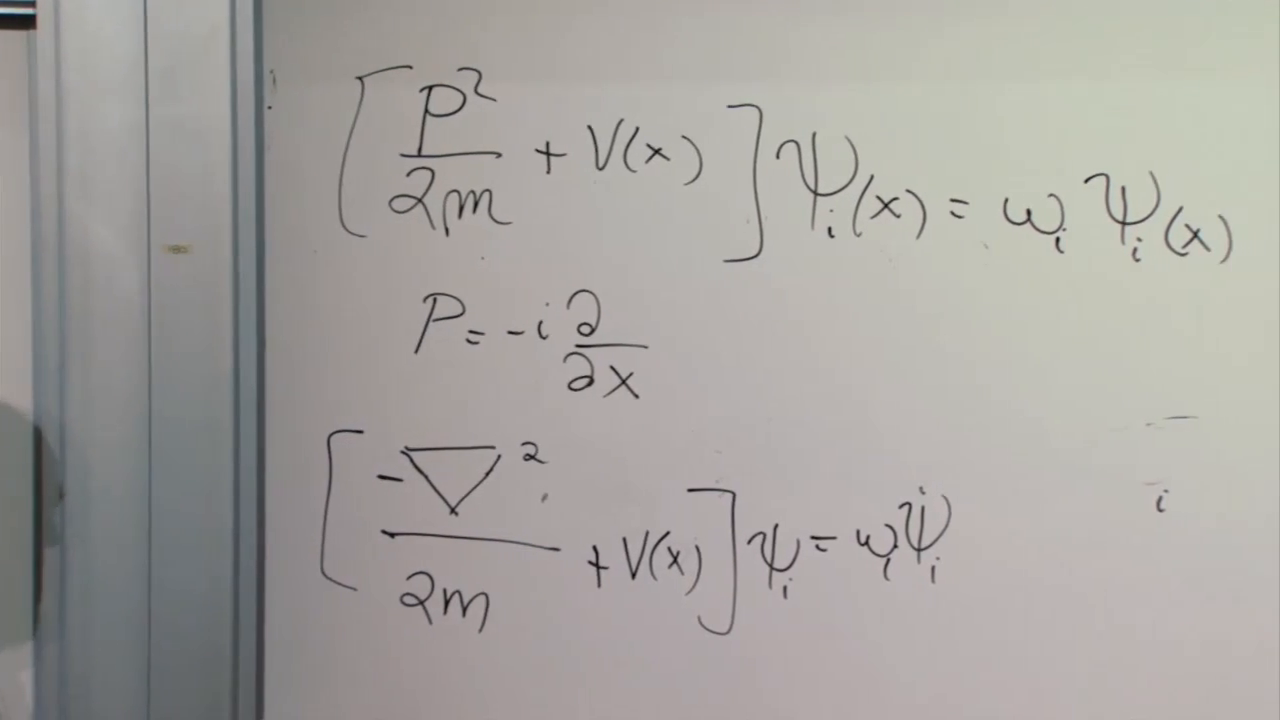
\includegraphics[width=0.94\linewidth]{lecture_07_frame_02.png}
\caption{El paso en la pizarra de \(p^2/(2m)+V(x)\) a la forma diferencial de la ecuación de autovalores de Schrödinger para una partícula. La Ecuación~\eqref{eq:l07-schrodinger-eigenvalue} es su reconstrucción depurada.}
\lectureframe{00:54:10}
\end{figure}

Para una función de onda arbitraria de una partícula normalizada, el valor esperado habitual es
\begin{equation}
\langle h\rangle_\psi
=\int dx\,\psi^*(x)h\psi(x).
\label{eq:l07-one-particle-energy-expectation}
\end{equation}
La fórmula para muchas partículas se sugiere al sustituir la función de onda minúscula por el campo con valores de operador. Esto todavía no es una demostración; es la conjetura cuya validez vamos a comprobar:
\begin{equation}
H=\int dx\,\Psi^\dagger(x)h\Psi(x).
\label{eq:l07-field-hamiltonian}
\end{equation}

\section{Escribir primero la respuesta y luego demostrarla}

Insertemos la Ecuación~\eqref{eq:l07-field-expansion} en el Hamiltoniano propuesto:
\begin{align}
\int dx\,\Psi^\dagger h\Psi
&=\int dx
\left(\sum_i a_i^\dagger\psi_i^*(x)\right)
h\left(\sum_j a_j\psi_j(x)\right) \\
&=\sum_{i,j}a_i^\dagger a_j
\int dx\,\psi_i^*(x)h\psi_j(x).
\label{eq:l07-h-expanded}
\end{align}
El operador diferencial \(h\) actúa sobre la función de onda \(\psi_j(x)\), que depende de \(x\), y no sobre el operador de modo \(a_j\). Por la ecuación de Schrödinger,
\begin{equation}
h\psi_j(x)=\omega_j\psi_j(x).
\end{equation}
En consecuencia,
\begin{align}
\int dx\,\Psi^\dagger h\Psi
&=\sum_{i,j}a_i^\dagger a_j\omega_j
\int dx\,\psi_i^*(x)\psi_j(x) \\
&=\sum_{i,j}a_i^\dagger a_j\omega_j\delta_{ij} \\
&=\sum_j\omega_j a_j^\dagger a_j.
\label{eq:l07-h-proof}
\end{align}
Esto es precisamente la Ecuación~\eqref{eq:l07-mode-hamiltonian}. La expresión local en términos del campo y la suma de las energías de todas las partículas son el mismo operador.

\begin{figure}[htbp]
\centering
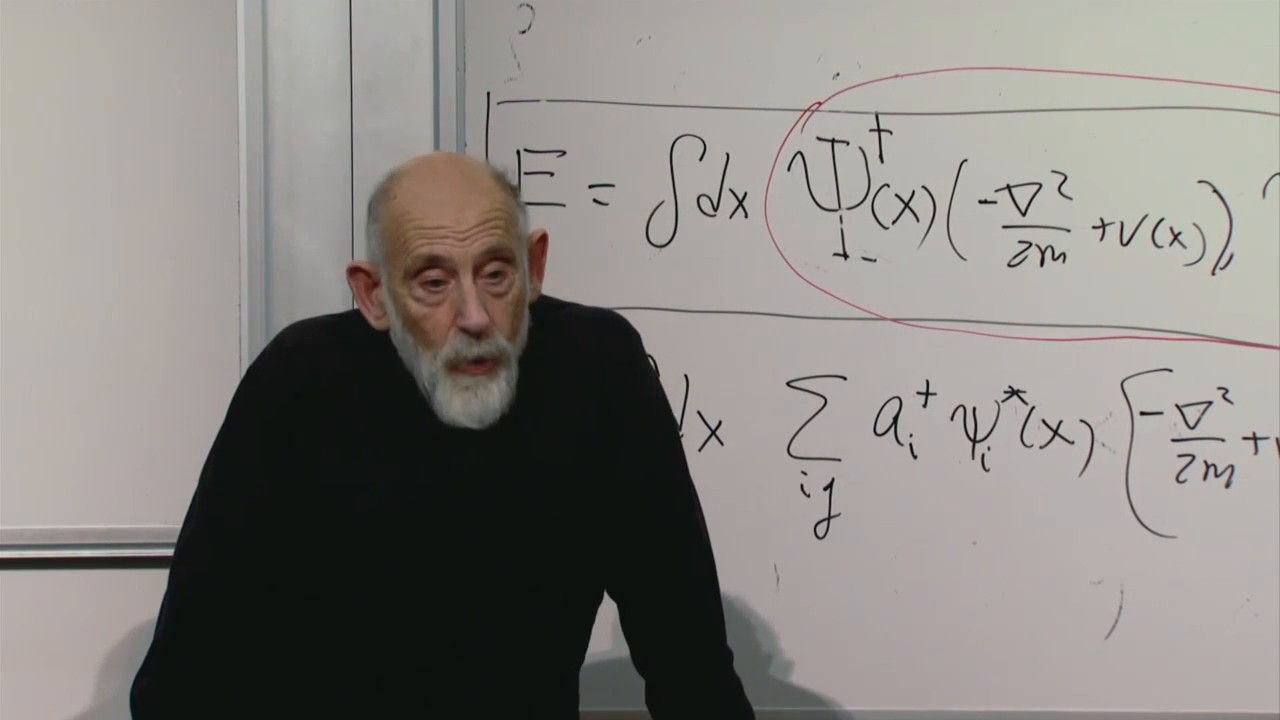
\includegraphics[width=0.94\linewidth]{lecture_07_frame_03.png}
\caption{El Hamiltoniano de campo destacado en la pizarra, con la demostración mediante la expansión en modos empezando debajo. Se conserva el fotograma de la clase como evidencia; las Ecuaciones~\eqref{eq:l07-field-hamiltonian}--\eqref{eq:l07-h-proof} restablecen el desarrollo algebraico completo.}
\lectureframe{01:05:34}
\end{figure}

En esta demostración no se ha conmutado ningún operador de creación a través de un operador de aniquilación. El orden \(a_i^\dagger a_j\) se mantiene de principio a fin. Los únicos objetos que se han desplazado libremente son las funciones de onda y sus autovalores, que son \(c\)-números.

\section{Por qué esto es un campo}

¿Por qué llamar campo a \(\Psi(x)\)? Porque es una cantidad con valores de operador definida en cada punto del espacio, y las combinaciones hermíticas o bilineales construidas a partir de ella son observables locales. La densidad \(n(x)\) y la expresión de energía local que aparece más adelante son dos ejemplos. La palabra no encierra ningún otro criterio matemático.

Este campo no es el campo electromagnético. Describe la especie no relativista que proporcionó los modos de una partícula y el Hamiltoniano \(p^2/(2m)+V\): por ejemplo, átomos lentos, neutrones, protones o electrones. Esas partículas son los cuantos de su campo correspondiente, en el mismo sentido estructural en que los fotones son los cuantos del campo electromagnético.

\begin{classroomqa}
\lecturetimestamp{01:02:45}
\audiencequestion{¿En qué momento, al pasar del sistema de muchas partículas a la fórmula anterior, aparece un campo?}
\lecturerresponse{Aparece en la Ecuación~\eqref{eq:l07-field-expansion}: \(\Psi(x)\) es un operador en cada punto espacial. Las derivaciones posteriores muestran que sus productos locales miden densidades de partículas y de energía. La dependencia de la posición, junto con el carácter de operador, es precisamente la estructura de campo que estamos construyendo.}
\end{classroomqa}

\section{Densidad local de energía}

La Ecuación~\eqref{eq:l07-field-hamiltonian} expresa la energía total como una integral sobre el espacio:
\begin{equation}
\begin{aligned}
H&=\int dx\,\mathcal H(x),\\
\mathcal H(x)
&=-\frac{1}{2m}\Psi^\dagger(x)\nabla^2\Psi(x)\\
&\quad+V(x)\Psi^\dagger(x)\Psi(x).
\end{aligned}
\label{eq:l07-hamiltonian-density}
\end{equation}
El integrando es una densidad local de energía natural para este Hamiltoniano. Su forma local no es única. Por ejemplo, una integración por partes sustituye el término cinético por
\begin{equation}
\mathcal H_{\rm kin}(x)
=\frac{1}{2m}\nabla\Psi^\dagger(x)\mathbin{\cdot}\nabla\Psi(x)
\label{eq:l07-kinetic-density}
\end{equation}
salvo por un término de contorno. Ambas expresiones dan el mismo Hamiltoniano total con las condiciones de contorno habituales. Esta es la pequeña ambigüedad mencionada en la clase.

\begin{classroomqa}
\lecturetimestamp{01:05:57}
\audiencequestion{¿Hay que integrar la densidad de energía sobre todo el espacio?}
\lecturerresponse{La integración sobre todo el espacio da la energía total. La integración sobre una región menor da la energía asignada a esa región, sujeta a la ambigüedad habitual al elegir una densidad local cuya integral sobre todo el espacio dé el mismo Hamiltoniano.}
\end{classroomqa}

\begin{classroomqa}
\lecturetimestamp{01:06:25}
\audiencequestion{¿En qué se diferencia la \(N_i\) mayúscula de la \(n_i\) minúscula en la fórmula de la energía?}
\lecturerresponse{\(N_i=a_i^\dagger a_i\) es un operador. El entero \(n_i\) es uno de sus autovalores en un estado de número de ocupación. Los operadores actúan sobre estados; sus autovalores son números ordinarios.}
\end{classroomqa}

\begin{classroomqa}
\lecturetimestamp{01:06:46}
\audiencequestion{¿Se puede escribir el propio Hamiltoniano de campo como un bra o un ket en la notación de Dirac?}
\lecturerresponse{No. Los bras y los kets representan vectores de estado y sus duales. El campo y el Hamiltoniano son operadores que actúan sobre esos estados. Un valor esperado como \(\langle\Phi|H|\Phi\rangle\) utiliza ambos tipos de objetos y no debe identificarlos.}
\end{classroomqa}

\section{Recuperar una partícula y acercarse a un campo clásico}

El formalismo ampliado contiene la mecánica cuántica ordinaria de una partícula. Restrinjamos el espacio de Fock a estados que satisfagan
\begin{equation}
N|\Phi\rangle=|\Phi\rangle.
\end{equation}
En ese sector, la construcción de campos reproduce todos los estados y todas las predicciones de una partícula. No hemos sustituido la teoría antigua; la hemos incorporado en un espacio que también puede describir cero, dos o un número arbitrario de partículas.

En el otro extremo, un modo ocupado por un número muy grande de bosones puede comportarse aproximadamente como una onda clásica. En estados coherentes o semiclásicos adecuados, el valor esperado
\begin{equation}
\Phi_{\rm cl}(x,t)=\langle\Psi(x,t)\rangle
\end{equation}
satisface la ecuación de aspecto clásico
\begin{equation}
i\partial_t\Phi_{\rm cl}(x,t)
=\left(-\frac{\nabla^2}{2m}+V(x)\right)\Phi_{\rm cl}(x,t)
\label{eq:l07-classical-schrodinger}
\end{equation}
para la teoría libre no relativista. La clase enuncia esta conexión, pero no la deriva. Es el puente entre una colección de cuantos y un campo ondulatorio: las ocupaciones grandes suprimen las fluctuaciones relativas y hacen que ciertos valores esperados se comporten clásicamente.

Por tanto, el formalismo es tanto un recurso para llevar la cuenta como una descripción física. Organiza todos los sectores de número de partículas, pero también recoge la interferencia, el entrelazamiento y la aparición de ondas clásicas a partir de partículas cuánticas.

\begin{classroomqa}
\lecturetimestamp{01:10:43}
\audiencequestion{¿Por qué se pueden manipular los operadores de creación y aniquilación dentro de la integral casi como si fueran números ordinarios?}
\lecturerresponse{Nunca se intercambiaron entre sí. Las funciones de modo ordinarias conmutan con ellos, y las derivadas actúan solo sobre esas funciones. Para pasar un operador de aniquilación a través de uno de creación habría que usar el conmutador, lo que podría añadir un término; la demostración no hace tal operación.}
\end{classroomqa}

\section{Un interludio sobre la notación de Dirac}

Parte de la confusión es histórica. Una función de onda de una partícula satisface una ecuación de ondas y se parece superficialmente a un campo clásico, aunque también es una amplitud de probabilidad. La teoría cuántica primitiva tuvo que separar esos papeles y luego explicar cómo los campos ondulatorios físicamente medibles, como el electromagnetismo, están formados por cuantos. El espacio de Fock y los campos con valores de operador resuelven el aparente conflicto.

La notación de Dirac hace que esta separación resulte excepcionalmente compacta. Un ket pertenece a un espacio vectorial, un bra a su dual, y al yuxtaponerlos se forma un producto interno. Entonces, la resolución
\begin{equation}
\sum_i|i\rangle\langle i|=\mathbf 1
\end{equation}
se vuelve casi autoexplicativa. La clase ilustra esto con una anécdota sobre la enseñanza de mecánica cuántica a matemáticos: el contenido matemático ya les resultaba familiar, pero la notación hacía tan transparentes las manipulaciones rutinarias que la estructura parecía nueva. La idea no es que a una disciplina le faltara el concepto. Es que una notación bien elegida puede hacer difícil confundir las operaciones permitidas.

Esta lección importa aquí. Ahora hay varios operadores distintos:
\begin{itemize}
\item \(h\) actúa sobre funciones de onda de una partícula como operador diferencial;
\item \(a_i\) y \(a_i^\dagger\) actúan sobre estados de número de ocupación en el espacio de Fock;
\item \(\Psi(x)\), \(\Psi^\dagger(x)\), \(N\) y \(H\) también actúan sobre el espacio de Fock.
\end{itemize}
La expansión de la Ecuación~\eqref{eq:l07-field-expansion} conecta los dos primeros contextos sin fundirlos.

\begin{classroomqa}
\lecturetimestamp{01:18:16}
\audiencequestion{¿Son los campos solo un formalismo para describir colecciones de partículas?}
\lecturerresponse{Son un formalismo, pero no uno vacío. Sus observables locales se pueden medir, y las partículas son partículas cuánticas con interferencia y entrelazamiento, no bolitas clásicas. Los operadores de campo codifican precisamente esas propiedades colectivas medibles.}
\end{classroomqa}

\section{Cautela relativista y una digresión sobre electromagnetismo}

La construcción hasta aquí es no relativista. El momento sigue siendo una buena etiqueta para las partículas en la física relativista, pero la posición de una partícula estrictamente localizada es mucho más delicada. Por consiguiente, una densidad local de número de fotones no suele ser un objeto tan limpio como \(n(x)\) en el caso no relativista. La densidad de energía sigue estando bien definida y es el observable local más seguro.

La clase ofrece una analogía electromagnética útil, explícitamente heurística. Combinemos los campos eléctrico y magnético en el vector complejo
\begin{equation}
\mathbf F=\mathbf E+i\mathbf B,
\qquad
\mathbf F^*=\mathbf E-i\mathbf B.
\label{eq:l07-riemann-silberstein}
\end{equation}
Entonces,
\begin{equation}
\mathbf F^*\mathbin{\cdot}\mathbf F
=\mathbf E^2+\mathbf B^2,
\label{eq:l07-em-density}
\end{equation}
que, en unidades convencionales, es proporcional a la densidad de energía electromagnética. Esto no es literalmente una densidad de probabilidad de fotones. Es mejor verlo como una variable de campo compacta cuyo módulo al cuadrado mide la densidad de energía o, informalmente, como una densidad de fotones ponderada por la energía de los fotones.

\begin{classroomqa}
\lecturetimestamp{01:19:10}
\audiencequestion{¿Se puede identificar la densidad de fotones con la intensidad del campo eléctrico?}
\lecturerresponse{Solo cualitativamente y con cautela. Para los fotones relativistas, el número local de partículas no es el concepto más adecuado. La afirmación sólida es que \(E^2+B^2\) es proporcional a la densidad de energía y que la combinación compleja \(\mathbf E+i\mathbf B\) expresa las ecuaciones de Maxwell en una forma parecida a la de Schrödinger.}
\end{classroomqa}

\begin{classroomqa}
\lecturetimestamp{01:20:09}
\audiencequestion{¿Por qué puede una partícula relativista tener un momento definido mientras que su posición es problemática?}
\lecturerresponse{El momento etiqueta de forma clara las representaciones relativistas de una partícula, mientras que la localización estricta entra en conflicto con la creación de partículas y con la descripción relativista mediante campos. Esta clase no desarrolla esa teoría; la advertencia señala el límite de la interpretación no relativista de la densidad que estamos usando.}
\end{classroomqa}

\section{Orden de operadores y constante del estado fundamental}

No se puede cambiar el orden de los operadores a la ligera. Para modos bosónicos,
\begin{equation}
a_i a_i^\dagger=a_i^\dagger a_i+1.
\end{equation}
Por consiguiente, sustituir el orden normal \(\Psi^\dagger h\Psi\) por el orden inverso \((h\Psi)\Psi^\dagger\), o por su versión integrada correspondiente, añade la contribución del conmutador. En una base de modos, es una suma aditiva de una unidad de energía cuántica por modo. Es la constante de energía del estado fundamental o de punto cero y, en un continuo, requiere regularización. La clase no aborda aquí ese asunto; solo advierte que los dos ordenamientos no son iguales.

\begin{classroomqa}
\lecturetimestamp{01:22:04}
\audiencequestion{¿Qué ocurre si se intercambian \(\Psi\) y \(\Psi^\dagger\) en el Hamiltoniano?}
\lecturerresponse{Hay que incluir su conmutador. Por tanto, invertir el orden añade una contribución independiente del estado al estado fundamental, en lugar de reproducir la misma expresión. El Hamiltoniano mostrado se mantiene en orden normal, \(\Psi^\dagger h\Psi\).}
\end{classroomqa}

\section{El momento como prueba final}

En los últimos minutos se repite una vez más la misma sustitución. Para una partícula,
\begin{equation}
\langle p\rangle_\psi
=\int dx\,\psi^*(x)\left(-i\partial_x\right)\psi(x).
\label{eq:l07-one-particle-momentum}
\end{equation}
Al reemplazar la función de onda por el campo, se obtiene el operador de momento total
\begin{equation}
P=\int dx\,\Psi^\dagger(x)\left(-i\partial_x\right)\Psi(x),
\label{eq:l07-field-momentum}
\end{equation}
o, en tres dimensiones,
\begin{equation}
\mathbf P=\int d^3x\,\Psi^\dagger(\mathbf x)
\left(-i\boldsymbol\nabla\right)\Psi(\mathbf x).
\end{equation}
Los campos transportan momento. Un láser suficientemente potente transfiere momento a una pared y ejerce una fuerza; en la descripción cuántica, ese momento del campo es la suma de los momentos de los fotones.

La ecuación~\eqref{eq:l07-field-momentum} es un operador, no un valor esperado. Dado un estado del espacio de Fock \(|\Phi\rangle\), se puede calcular
\begin{equation}
\langle P\rangle_\Phi=\langle\Phi|P|\Phi\rangle.
\end{equation}
Para formar un valor esperado se necesitan tanto un operador como un estado. Confundir el observable con su promedio borraría precisamente la distinción que la exposición se ha esforzado por establecer.

\begin{classroomqa}
\lecturetimestamp{01:26:02}
\audiencequestion{¿El momento del campo que se muestra es ya el momento promedio?}
\lecturerresponse{No. Es el operador hermítico que representa el observable. Para obtener un valor esperado, se proporciona un estado y se intercala el operador entre su bra y su ket; una medición aún puede fluctuar alrededor de ese promedio.}
\end{classroomqa}

Este es el punto natural para detenerse. Partiendo de las partículas, hemos construido campos locales de creación y aniquilación, los hemos usado para contar partículas y hemos reescrito la suma de las energías y los momentos de una partícula como operadores de campo. El siguiente paso no consiste en otro cambio de notación, sino en hacer que los operadores de campo representen procesos físicos: partículas que se desintegran, partículas que se dispersan y especies que se transforman unas en otras.
